\section{\aimThree}

\note[enumerate]{
    \item Aim 1\&2 are about what we can do with best-in-class models; aim 3 is about simplifying the model / making more biologically compatible. Less complexity but simpler. How close in performance can we get to ``gold standard" model from Aim 1 \& 2?
    \item First, we introduce prior work on functional motif discovery via optogenetics.
    \item Next, I will discuss possible biological priors and constraints
}

\begin{frame}{\qThree}
    \textbf{Hypothesis:} Enforcing causal biological constraints will improve model performance while aiding interpretatation
    \begin{enumerate}
        \item Requiring model to predict \emph{in situ} hybridization allows for interpretation of cell-type contribution to dynamics
        \item Template-based representations allow for unsupervised learning of purported circuit motifs
    \end{enumerate}
\end{frame}

\begin{frame}{ \emph{in situ} cell type identification }
    \begin{center}
        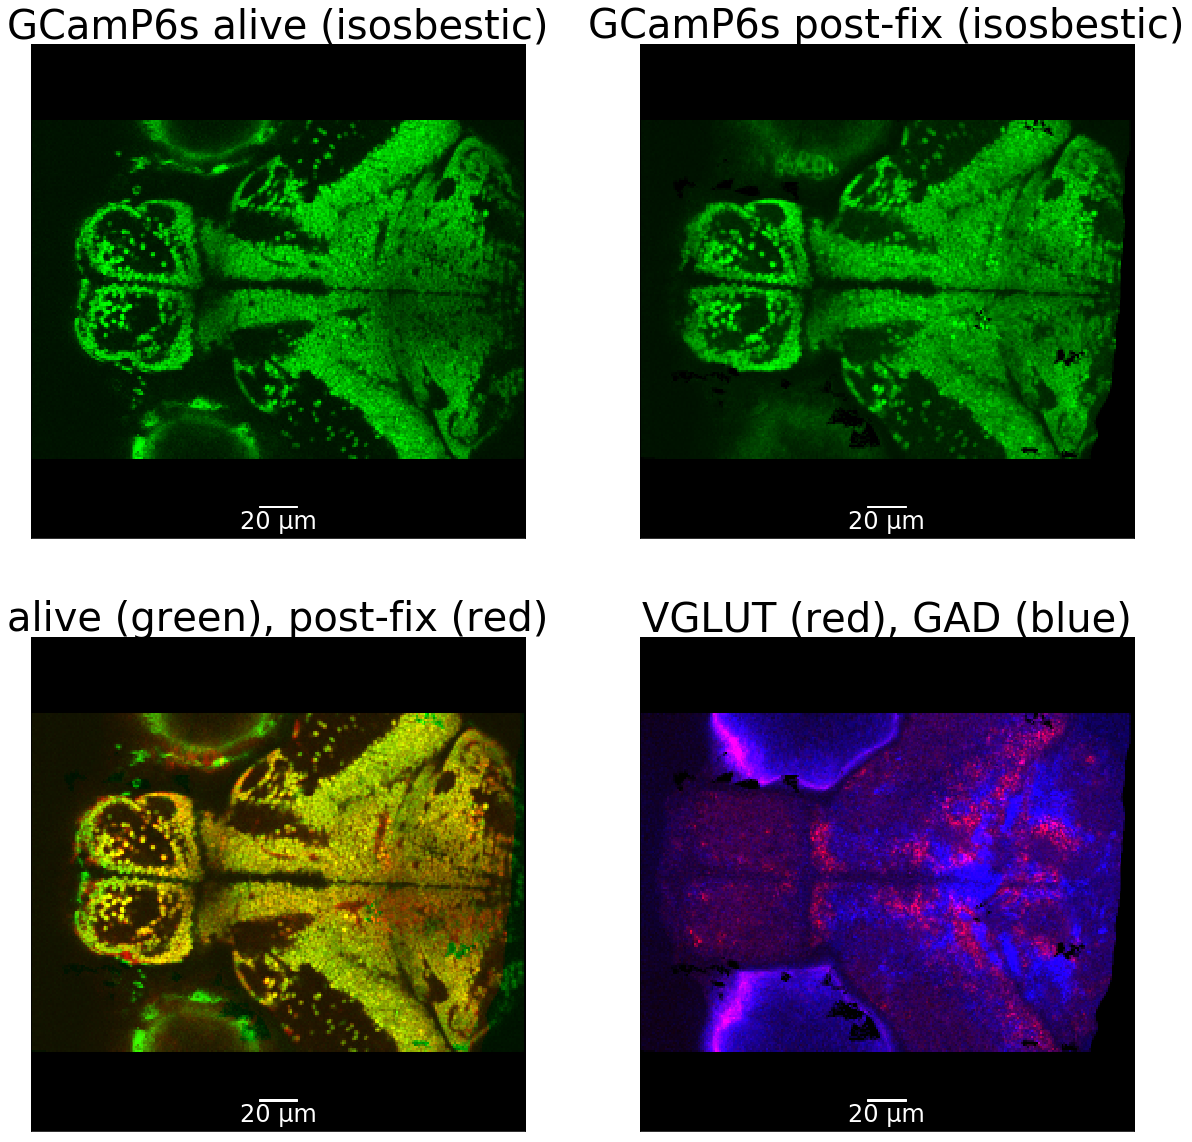
\includegraphics[height=\textheight]{media/ish_stain.png}
    \end{center}
    \note{Talk about colored graphs, predicting cell type,}
\end{frame}{}

\begin{frame}{ \emph{in situ} cell type identification: attempts to date}
    \begin{itemize}
        \item Thus far, including \emph{in situ} data has not helped with functional prediction
        \item Thus far, including \emph{in situ} data has not succeeded in predicting cell type (attemted conv-GRU and conv-LSTM)
        \item Additional architectures should be explored / debugged
    \end{itemize}
\end{frame}{}

\begin{frame}{ Network motifs }
    \begin{multicols}{2}
        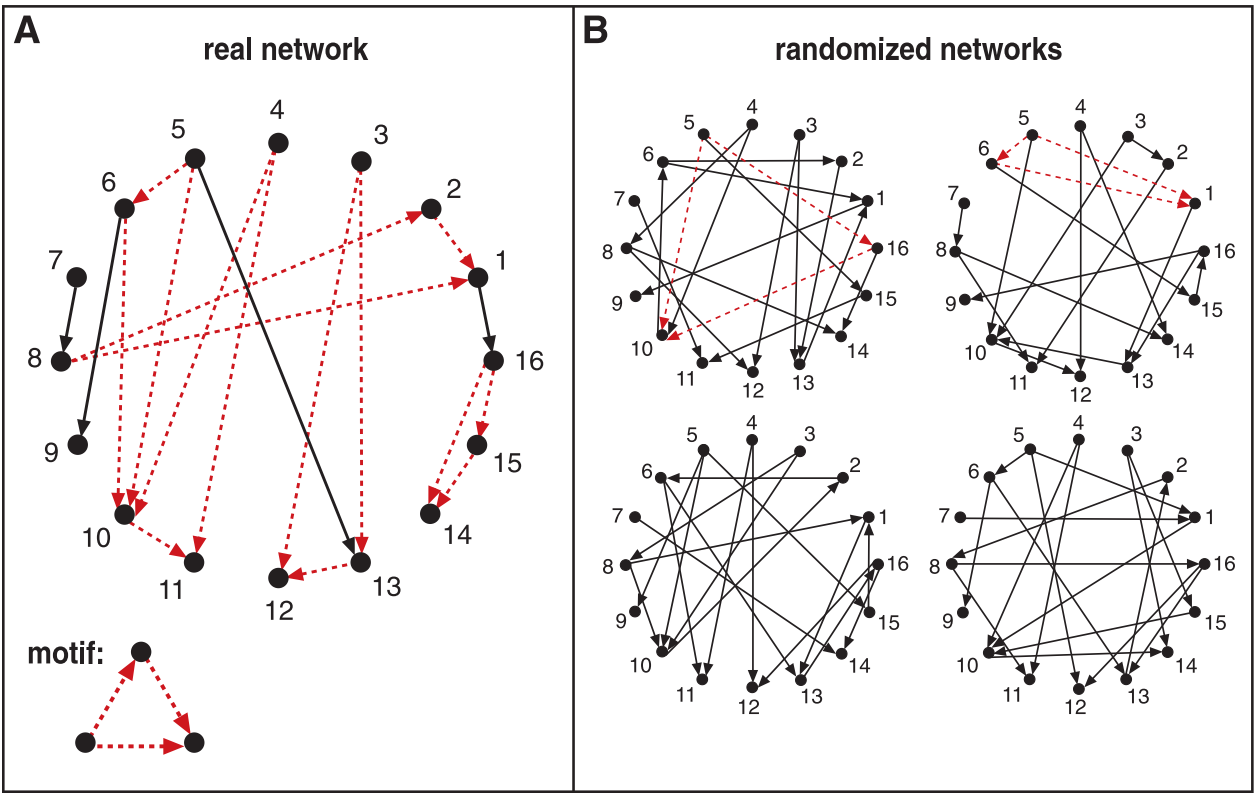
\includegraphics[width=0.5\textwidth]{media/motif_schematic.png}
        Schematic illustrating an over-represented motif\nakedfootnote{Milo et al 2002}
        \note{For a stringent comparison, we used random- ized networks that have the same single-node characteristics as does the real network: Each node in the randomized networks has the same number of incoming and outgoing edges as the corresponding node has in the real network.

        }

        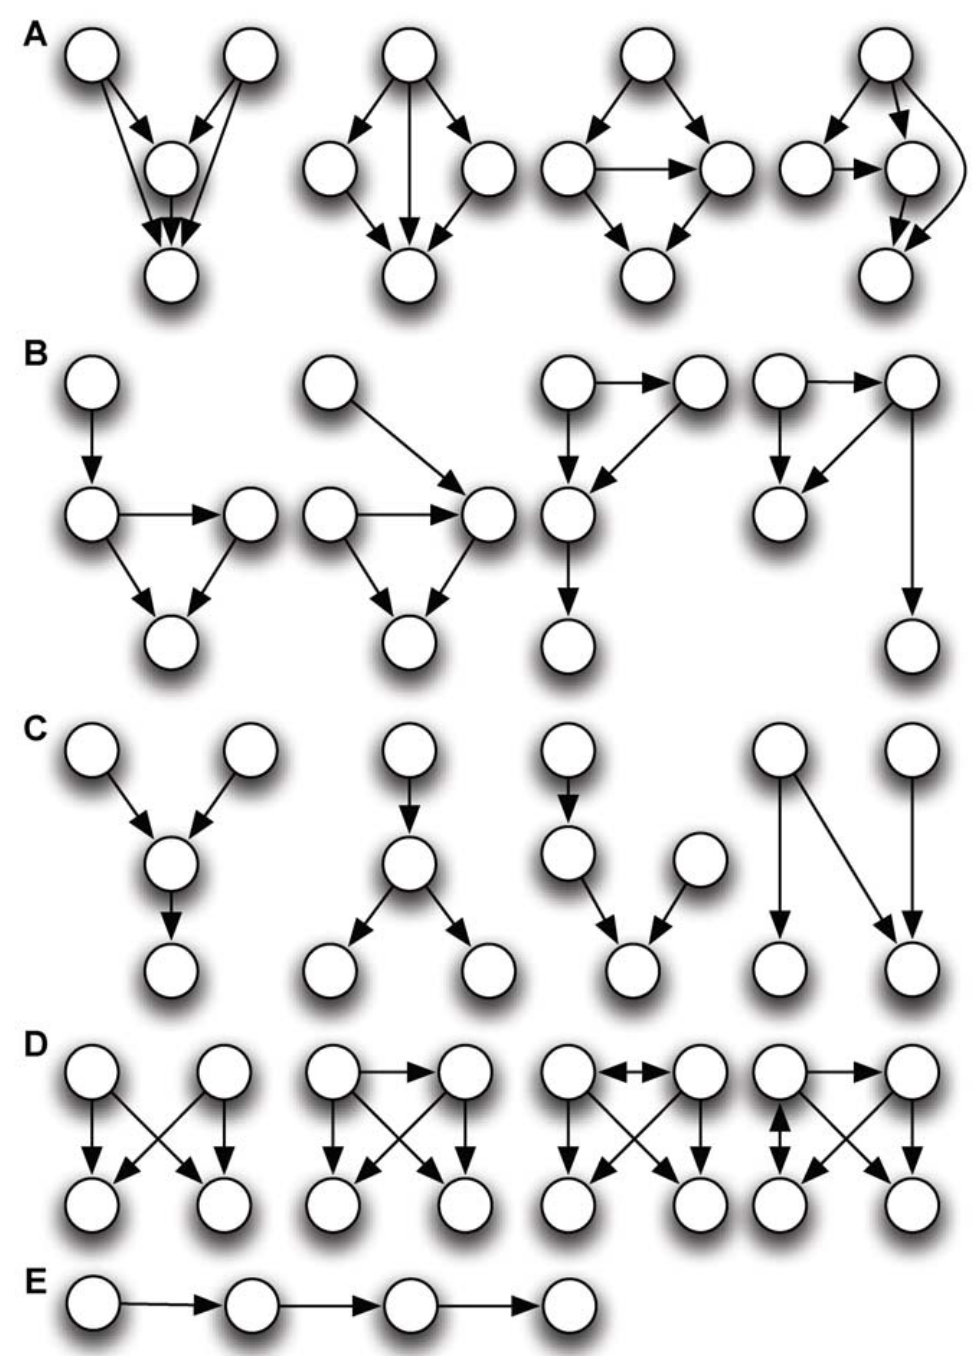
\includegraphics[height=0.7\textheight]{media/celegans_motifs.png}
        Over-represented motifs from \emph{C. elegans} connectome\nakedfootnote{Qian et al 2011}

        \note{A: nested feed-forward motifs, B: feed-forward motifs with entry and exit, C: integrations and bifurcations, D: bi-fan motif with or without coupling of the inputs, and E: linear chains.}
    \end{multicols}
\end{frame}{}

% \subsection{Cell type}
% \subsection{Circuit motifs}
